\documentclass[hidelinks,12pt]{report}
\usepackage[utf8]{inputenc}
\usepackage{float}

\usepackage[margin=1.2in]{geometry}
\usepackage[T1]{fontenc}
\usepackage{graphicx}
\usepackage{pdfpages}
\usepackage{mathtools}
\usepackage{hyperref}
\usepackage{mathtools, bm}
\usepackage{amssymb, bm}
\usepackage{indentfirst}
\graphicspath{ {images/} }
%indent
\setlength{\parindent}{1em}
\setlength{\parskip}{1em}
%figures at the begining of page
\makeatletter
\setlength{\@fptop}{0pt}
\makeatother
%for tables
\newcommand{\bigcell}[2]{\begin{tabular}{@{}#1@{}}#2\end{tabular}}

\newcommand{\ml}[1]{\textcolor{blue}{ Mathieu : #1}}

\begin{document}
\chapter{Ranking against the instrument class and the playing technique}
\section{clustering the samples.}

\ml{USE PRESENT TIME ALWAYS AND AVOID USING WE DID THIS, WE DID THAT !!}

In the first part of the study, the following ranking problem was studied. We have 25119 musical extraction of different solo instruments playing different techniques of play. Those samples will be clustered in three different ways: 
\begin{enumerate}
\item \textbf{ 16 classes of instruments.}\\
In the first labeling type the samples are classified based on the instruments they are played with. Since the database provided contains 16 different instruments, the samples were divided in 16 different clusters.
\item \textbf{32 classes of instruments with variation.}\\
To add some complexity to the instrument clustering and to further test the stability of the code, an additional variation to the instruments clustering was considered. So for example, a sample played without mute will be given different label than a sample played by the same instrument with mute.
\item \textbf{498 classes of instrument with different playing techniques.}
The last clustering and the most complex ranking problem to solve, is considering that two samples played with different techniques will have different labels even if they are being played by the same instrument. Thus there would be 498 different labels in this clustering.\\

\end{enumerate}
\section{Experimental procedure}
The experimental procedure is composed of two parts. The first one computes the features based on one of the two representations: MFCC or scattering (with different parameters). In the second part the ranking metrics before will be computed before and after processing the data in the feature space.\par
In the first part, the use of the two representations is done as follows : using a fixed length window of calculation we obtain a certain number of temporal features based on the length of the signal. Then, by averaging along the time axis, only one vector of features by audio file is left.In this space, the Euclidean distance is chosen to compute the distances between observations.\\ 
For the second step, the distance computation is done using pairwise Euclidean distance measure. Many form of processing in the feature space have been tested and only the one that proved efficient will be shown here and presented in further details in later chapters :
\begin{itemize}
\item Standardization.
\item High or low variance filtering.
\item Projecting into symmetrical data \ml{whitening, provide reference of Vincent's paper if you do not know which one, ask vincent} 
\item Large Margin Nearest Neighbor.\cite{W09}\\
\end{itemize}

After processing the data, the pairwise Euclidean distance will be computed, which will be evaluated using the two ranking metrics that are the basis of our performance analysis, namely the MAP and P@k metrics.

\ml{tu parles plusieurs fois de la distance euclidienne, alors qu'elle n'est calculé qu'une fois, a la limite tu peux simplement dire que les métriques sont calculés dans l'espace euclidien apres post traitements eventuels}

\begin{figure}[t!]
  
  \centering
	    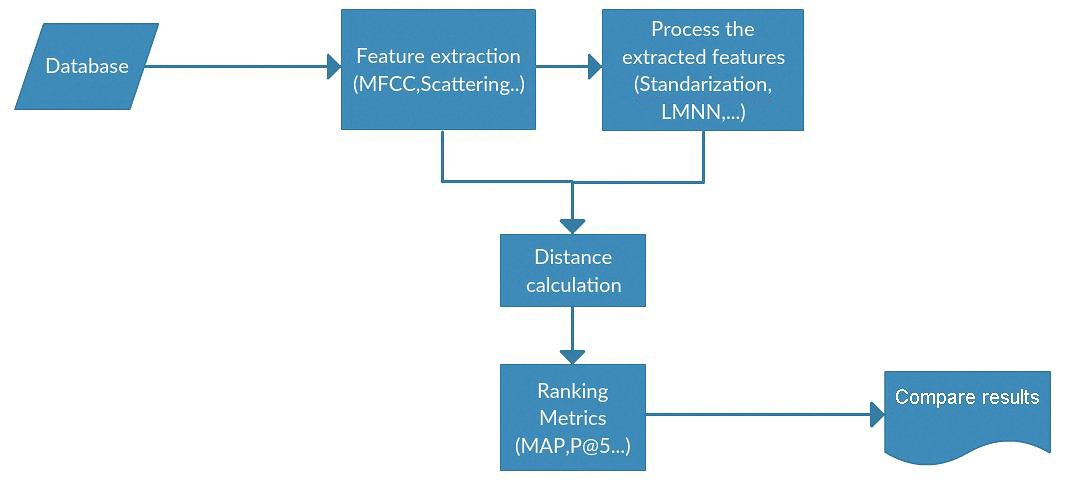
\includegraphics[width=1\textwidth]{experimental_procedure}
    \caption{Experimental procedure \ml{hard to read, try pgf/tikz for generate block diagram or at least use bigger bold and black fonts} }
    \label{expermient}
\end{figure}
The following sections will follow the same scheme presented in figure \ref{experiment}. First will be the feature extraction procedure, following will be the methods of processing in the feature space. At the end, The performance will be analyzed using the distance computation and ranking metrics.

\section{Feature extraction}
In this section the two methods of feature extraction used studied in this report will be presented alongside the motivation and the algorithm of computation. We will start first by the Mel Frequency Cepstral Coefficients and then the scattering representation. 
\subsection{Mel Frequency Cepstral Coefficients MFCC}
The MFCC (Mel Frequency Cepstral Coefficients)  became famous with the rise of speech recognition systems. The MFCC are able to mcast a spoken stream in a compact and meaningful space. Those coefficients contains most of the information needed for processing spoken audio streams. They are still found in most of the audio processing applications. In the musical domain MFCC has been widely used for music genre classification.\\ The biggest limitation of the MFCC, as we will see in details, is its inability to encode large time scale variation.

\subsubsection{Algorithm and motivation}
\begin{figure}[t!]
  
  \centering
	    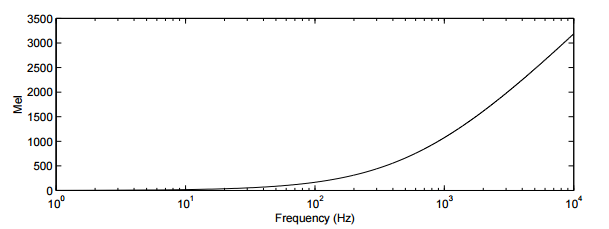
\includegraphics[width=0.7\textwidth]{melscale}
    \caption{Mel scale }
    \label{mel}
\end{figure}
The extraction of the MFCC features is divided into 5 steps as presented in figure \ref{mfcc}. In this part, Each step is presented along with the motivation and the limitation it provides.
\begin{figure}[t!]
  
  \centering
	    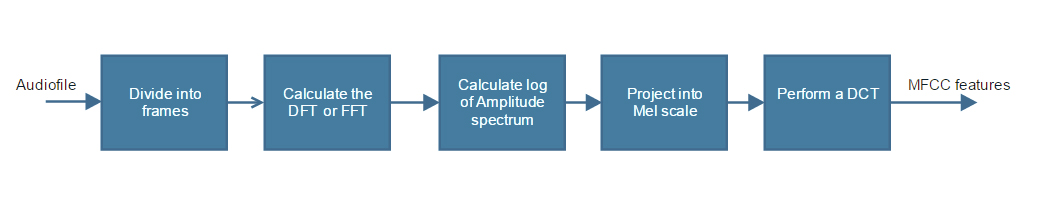
\includegraphics[width=1\textwidth]{MFCC2}
    \caption{Procedure of MFCC feature extraction }
    \label{mfcc}
\end{figure}
\begin{enumerate}
\item \textbf{Frame division} \\
The first step is to divide the waveform into equal spaced frames in the time domain. The split is obtained by applying a windowing function at fixed time intervals. This step is motivated by the fact that audio signals (music and speech) \ml{are -> can be considered as} statistically stationary for a short period of time. The limitation of this step is related to the length of the windowing function. It is proven that the best results are obtained for a window function length between 25 and 40ms. The longer the frame the bigger the variation of the signal in each frame and this will lead to a loss of information. 

\item \textbf{DFT or FFT computation\\}
The discrete Fourier transform (or fast Fourier transform) is used to project from the time domain to the frequency domain. By using the Fourier transform we obtain the amplitude of the spectrum and thus we lose knowledge of the phase. The motivation of computing the MFCC, is that the information provided to the brain by the cochlear is the amplitude of the frequencies(1.3.1).
\item \textbf{LOG of amplitude spectrum computation}\\
We take the log of the spectrum amplitude obtained by the Fourier transform. This step is motivated by the human perception of the sound loudness. The loudness of the sound is perceived by human in a logarithmic way : we need to put 8 time more energy to achieve a hearing experience of double loudness. 
\item \textbf{Mel scale projection}
In this step we aim to reduce the space and smooth the spectrum by applying a mapping from the log amplitude spectrum to the Mel frequency scale. This mapping is logarithmic for high frequencies(higher than 1KHZ) and linear for low frequencies(below 1KHZ). The scale is motivated by the fact that we do not perceive pitch in a linear way. The mapping allow us to reduce the space to n features space, where n can vary up to 40.
\item \textbf{DCT computation}
We are now left with 40 highly correlated features and most of them containing unnecessary information. To achieve the decorrelation and extract the interesting features a Discrete Cosine Transform is applied and only the first 12 of the 27 features are kept. \ml{give evidence why we do each step}
\end{enumerate}
\subsubsection{MFCC parameter choice}
Before we started our study on the MFCC we had to tune the values of different parameters, the default factors for the MFCC were proven to be the best.
\subsubsection{How the results were obtained}
To extract the features, a function called SaveAllDattaCoeffplusload.m was written. This function search in the folder of the database for the audio files. For each audio samples it either extract the MFCC or the scattering coefficients and average in time to obtain one vector of features per audio sample. It also gives for each audio file three different labels, the first one based on which instrument is playing, the second one is based on which instrument is playing plus the fact that it has variation or not, and the last one is based on the playing technique. At a result we will obtain one matrix of $M*N$ where M is the number of audio files and N is the number of feature extracted.\\
The Matlab function pdist was applied to compute the pairwise distances between each two observations. This will result in a $M*M$ matrix. We than use this matrix alongside each vector of labels(16 class of instruments, 32 class of instruments with variations and 498 class of technique of play) as inputs of the function rankingmetrics.m to compute the MAP and the P@5.\\
The results are divided into three tables with the number of class varying from 16,32 to 498. Two variations of the mfcc are shown with the first one is by taking 12 features out of the 27 and the other is with taking all the 27 features. The last one is by taking the features in the mel space without applying the DCT(40 features).\\

\ml{while reporting results, avoid speaking of the actual implementation, so do not porvide reference to code}

\begin{table} [H]
\begin{center} 
\ 
 \setlength{\tabcolsep}{.16667em} 
\begin{tabular}{ | l | l | l | }
features  & map & pat5  \\ 
\hline 
mfcc 12/27  & 22.66 & 85.93  \\ 

mfcc 27/27  & 19.72 & 85.24  \\ 

mel &  16.48 & 62.90 \\ 

\end{tabular} 
\end{center} 
\caption{Results of the study performed on the MFCC features. Labels taken as 16 class of instruments} 
\label{you} 
\end{table} 


   
\begin{table} [H]
\begin{center} 
\ 
 \setlength{\tabcolsep}{.16667em} 
\begin{tabular}{ | l | l | l | l |}
features  & map & pat5 \\ 
\hline 
mfcc 12/27  & 20.84 & 83.98  \\ 
 
mfcc 27/27 & 17.87 & 82.85  \\ 

mel  & 14.72 & 60.26  \\ 

\end{tabular} 
\end{center} 
\caption{of the study performed on the MFCC features. Labels taken as 32 class of instruments with variation} 
\label{you} 
\end{table} 

\begin{table} [H]
\begin{center} 
\ 
 \setlength{\tabcolsep}{.16667em} 
\begin{tabular}{ | l | l | l |  }
features  & map & pat5  \\ 
\hline 
mfcc  & 8.24 & 43.95 \\ 

mfcc 27/27  & 8.85 & 43.96 \\  
mel  & 5.74 & 32.90  \\ 

\end{tabular} 
\end{center} 
\caption{Results of the study performed on the MFCC features. Labels taken as 498 class of techniques of play}  
\label{you} 
\end{table} 
The best results were proven to be by taking 12 out of the 27 MFCC coefficients.

\subsubsection{MFCC features preprocessing}
When dealing with a big space of data, Usually a preprocessing technique should be applied before proceeding to use a learning algorithm. This usually proves to be efficient, and there are  different techniques of normalization that can be tested for example :   The effect of preprocessing the MFCC features was tested using the standardization technique.\\
\textbf{Feature standardization :}
In feature standardization, each feature is taken independently and treated in the following way : \\
for each dimension we
\begin{itemize}
\item Compute the mean.
\item Substract the resulting mean.
\item Compute the standard deviation.
\item Divide by the standard deviation.
\end{itemize}
This technique is widely used as a preprocessing for MFCC, since it removes the effect of the DC component that overshadows the space. The result of applying the standardization is shown in the tables below.
\begin{table}[H] 
\begin{center} 
\ 
 \setlength{\tabcolsep}{.16667em} 
\begin{tabular}{|l|l|l|} 
metrics & map & pat5  \\ 
\hline 
raw & 22.66 & 85.93  \\ 
standardize & 24.22 & 86.89  \\ 
 
\end{tabular} 
\end{center} 
\caption{Comparison between MFCC before and after standardization for the 16 classes of instruments} 
\label{me} 
\end{table}

\begin{table}[H]
\begin{center} 
\ 
 \setlength{\tabcolsep}{.16667em} 
\begin{tabular}{|l|l|l|} 
metrics & map & pat5 \\ 
\hline 
raw & 20.84 & 83.98 \\ 
standardize & 22.29 & 85.12  \\ 

\end{tabular} 
\end{center} 
\caption{Comparison between MFCC before and after standardization for the 32 classes of instruments with variation} 
\label{me} 
\end{table} 

\begin{table}[H]
\begin{center} 
\ 
 \setlength{\tabcolsep}{.16667em} 
\begin{tabular}{|l|l|l|} 
metrics & map & pat5  \\ 
\hline 
raw & 8.24 & 43.95  \\ 
standardize & 8.78 & 45.19  \\ 

\end{tabular} 
\end{center} 
\caption{Comparison between MFCC before and after standardization for the 498 classes of playing techniques} 
\label{me} 
\end{table}
As it is shown in the tables, the results indicate that standardization yields to a slight performance while performed in the MFCC feature space.

\ml{too few comments, each table shall have at least a sentence.}

\subsection{The Scattering transform}
\begin{figure}[t!]
  
  \centering
	    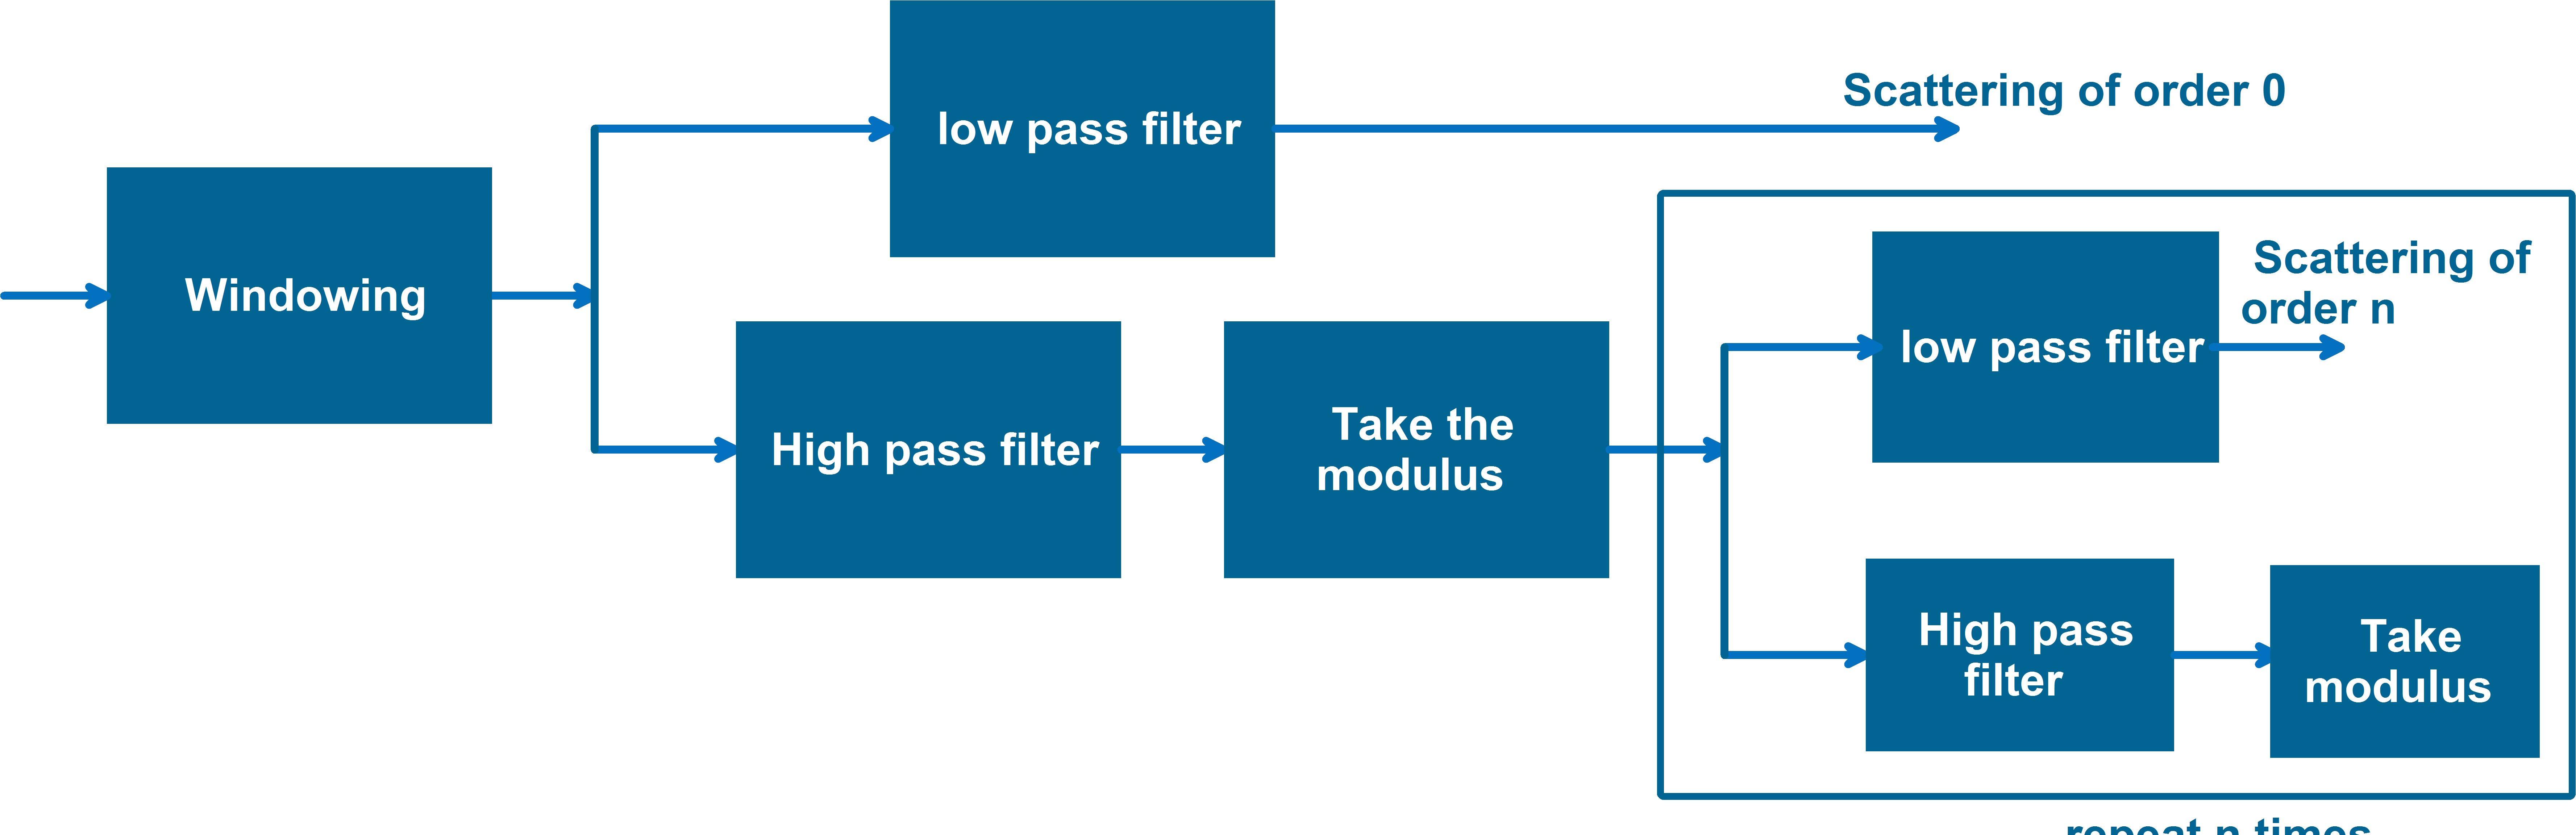
\includegraphics[width=1\textwidth]{scattering}
    \caption{Scheme of the scattering transform procedure }
    \label{scat}
\end{figure}
The second feature extraction method that was studied is the scattering transform. This method achieves signal decomposition using multiple wavelet transform alongside modulus operators. Figure \ref{scat} shows a scheme of how the procedure of extracting the scattering coefficients works. 

\ml{please indicate that the use of the scattering transform is recent and under active research}

\begin{enumerate}
\item We first divide the audio samples into frames by using a windowing function. Those windows can vary from multiples of 10 milliseconds to the order of multiples of 100 milliseconds.  
\item Apply to the frames a low pass filter. The output of that filter will be the scattering of order n.
\item Apply to the frames a high pass filter. Take the modulus of the output and replace the frames with the output of this step. \ml{this is not a high pass filter, this is a wavelet filter bank}
\item Repeat the step 2 and 3 n times. For audio signals scattering of order 2 is enough to represent the data.
\end{enumerate}
\subsubsection{Reducing variance of the representation}
Audio signals contains information that dose not alter the perception of sounds by human. And for tasks such as instrument identification, those information are not important. Such information are : 
\begin{itemize}
\item Translating an audio signal in time will not alter the perception of this sound by humans. Audio signals \ml{perception} are thus \ml{largely} time invariant. \ml{Indded}, discarding the information of time location will not alter the identification of instruments or \ml{techniques of play -> playing techniques}. The representation $\Phi$ will thus have the following property $\Phi(x(t-c))=Phi(x(t))$.
\item Other information that can be discarded are the one related to time warping. Time warping can be considered as shifting the signal by a factor that is time dependent. Audio signals are invariant to small scale time warping. What is needed from the representation is not to be time warping invariant $\Phi (x(t-c(t)))=\Phi(x(t))$ rather to be stable to time warping. This can be seen as a lipschitz continuity condition : $$||\Phi (x(t-c(t)))-\Phi(x(t))|| \leq C||x||||c'||_{\infty}$$
\end{itemize}
The scattering transform is based on a wavelet transform. To better understand how the time shifting and stability to deformation are obtained, let us look at each of the figure \ref{scat} block alone.\par
\textbf{Low pass filter :}
To achieve stability to time shifting, an average in time is applied. This average is achieved by applying a low pass filter. At the first step all the information is lost by this low pass filter, and the result is 0 for scattering of order 0. This same averaging will be applied again before the output of each order to insure time invariance.\par
\textbf{High pass filter:}
Since a lot of the information is lost in the low pass filter, A series of high pass filters is applied to encode the lost information. To ensure stability to time warping, The high pass filters used are wavelet functions. The use of wavelet is motivated by the fact that at low frequency they have high frequency resolution and at high frequency the have low frequency resolution. This will guarantee overlapping at high frequencies between a signal warped in time and a signal not warped.\par
\textbf{Take the modulus}
By applying a low pass filter again to the output of the high pass filters, again an average of 0 is obtained. To avoid this, a non linearity should be introduced. In the scattering transform, the best non linearity to be considered is by taking the modulus.\par
\textbf{Cascading}
At each step, only the output of the low pass filter is taken. This means that at each step, a loss of high frequency information is forced. To obtain those information again, a cascade High pass filter and low pass filter is done until the loss of information is not significant anymore. To further demonstrate the importance of second order coefficients the following examples will be discussed.\par
\begin{figure}[t!]
  
  \centering
	    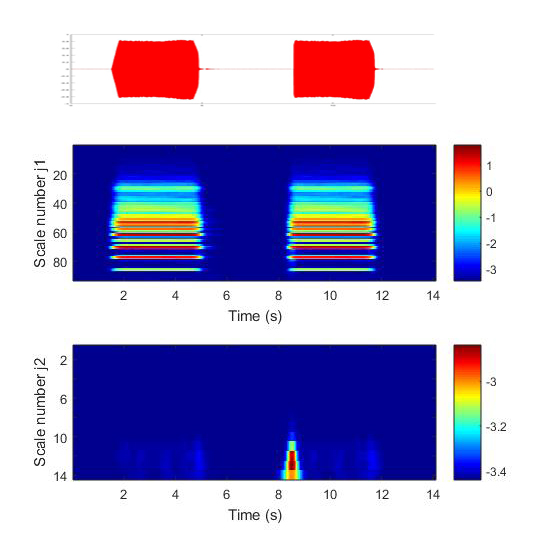
\includegraphics[width=0.6\textwidth]{att}
    \caption{[a.] Variation of amplitude in time of two samples one with smooth attack and the second one with sharp attack. [b.] scattering of order 1 of both signals [c.] scattering of order 2 of both signals }
    \label{attack}
\end{figure}
\subsubsection{Examples presenting the importance of second order}
In the figure \ref{attack} two audio samples are presented of an accordion playing the note A3. The first sample is with a soft attack and the second one is with a sharp attack. Since in the first order coefficient, the resolution of high frequency is low, no information related to the attack can be found easily and the two samples can be confused. \\
By looking at one of the second order coefficients corresponding to one of the high frequencies. The attack can be clearly found. And the difference between the two samples can be easily done.\par
In the figure \ref{vib} the same analysis can  be made. This time The first sample present an audio without vibrato, while the other one present the same audio with vibrato. Since the first order coefficients does not have high resolution for high frequencies, the frequency of the vibrato is lost. By taking the second coefficient of one of the first order feature, the frequency of the vibrato is clearly visible as a frequency not varying in time.
\begin{figure}[t!]
  
  \centering
	    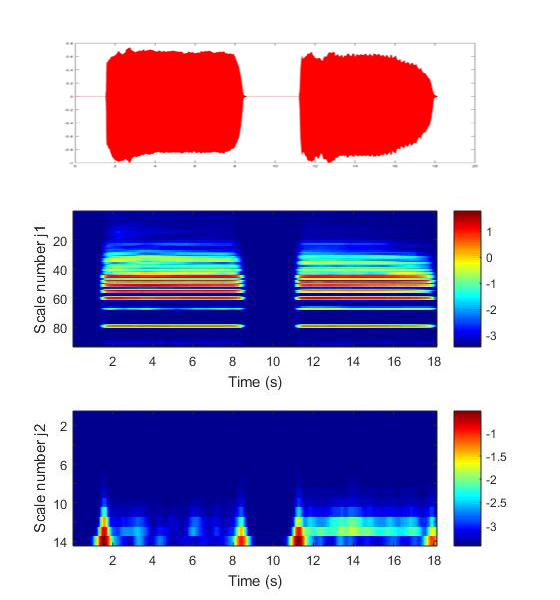
\includegraphics[width=0.6\textwidth]{vib}
    \caption{[a.] Variation of amplitude in time of two samples one without vibrato and the second one with vibrato. [b.] scattering of order 1 of both signals [c.] scattering of order 2 of both signals }
    \label{vib}
\end{figure}
\subsubsection{Results of varying the length of the windowing function T}
The impact of taking smaller window time on the output of the ranking metrics. The test was performed on the 16,32 and 498 labeling variations. The results are given in the three following tables.
\begin{table} [H]
\begin{center} 
\ 
 \setlength{\tabcolsep}{.16667em} 
\begin{tabular}{ | l | l | l | l | l |}
features  & map & pat5  \\ 
\hline 
scattering T=25ms & 18.07 & 72.79  \\ 
 
scattering T=128ms  & 16.79 & 70.47  \\ 

scattering T=250ms  & 16.49 & 70.40  \\ 

\end{tabular} 
\end{center} 
\caption{Table comparing the results of applying metric ranking to different window length for the scattering transform considering 16 class of instruments} 
\label{you} 
\end{table}

\begin{table} [H]
\begin{center} 
\ 
 \setlength{\tabcolsep}{.16667em} 
\begin{tabular}{ | l | l | l | l | l |}
features & map & pat5 \\ 
\hline 
scattering25  & 16.29 & 70.17  \\ 

scattering128 & 15.18 & 67.21  \\ 

scattering250  & 14.89 & 67.05  \\ 

\end{tabular} 
\end{center} 
\caption{Table comparing the results of applying metric ranking to different window length for the scattering transform considering 32 class of instruments with variations} 
\label{you} 
\end{table} 


\begin{table} [H]
\begin{center} 
\ 
 \setlength{\tabcolsep}{.16667em} 
\begin{tabular}{ | l | l | l | l | l |}
features & map & pat5  \\ 
\hline 
scattering25 &  7.79 & 40.17  \\ 

scattering128  &  6.66 & 37.38 \\ 

scattering250  &  6.46 & 37.07 \\ 
 
\end{tabular} 
\end{center} 
\caption{Table comparing the results of applying metric ranking to different window length for the scattering transform considering 498 class of technique of play} 
\label{you} 
\end{table}

\ml{again, each table have to be commented}

\subsubsection{Preprocessing the scattering features}
As for the MFCC, the normalization that was tested on the scattering features is the standardization. Another type of preprocessing was applied, that will be referred to as std and median method.\par
\textbf{Std and median method :} The scattering features present a lot of variability in its factors, with some of the factors being irrelevant to the process. To remove those factors and reduce the space, a study of variance should be done. The variance of each feature alone is computed, and sorted by growing values. The accumulated sum is then computed and either the high or the low variances will be discarded. In both cases an improvement was noticed but the best result was achieved with only leaving 83\% of the high frequencies. This is the std part of the method. \\
The second part is to divide by the vector of median (the median of each feature is computed alone). The feature space is then divided by the median. This will make the space \ml{the distribution of the features not the space} symmetrical and close to Gaussian.\\
The effect of the standardization and the std and median method is represented in the three tables below.

\ml{remove space when possible}

\begin{table} [H]
\begin{center} 
\ 
 \setlength{\tabcolsep}{.16667em} 
\begin{tabular}{ | l | l | l | l | l |}
metrics & map & pat5  \\ 
\hline 
raw & 16.49 & 70.40  \\ 
standarize & 19.31 & 78.98 \\ 
stdandmedian & 30.73 & 93.87 \\ 
 
\end{tabular} 
\end{center} 
\caption{Table comparing the results of applying metric ranking to different technique of preprocessing on a scattering with T=250ms considering 16 class of instruments} 
\label{you} 
\end{table}

\begin{table}[H]
\begin{center} 
\ 
 \setlength{\tabcolsep}{.16667em} 
\begin{tabular}{|l|l|l|} 
metrics & map & pat5  \\ 
\hline 
raw & 14.89 & 67.05 \\ 
standarize & 17.52 & 75.13  \\ 
stdandmedian & 28.07 & 90.94  \\ 

\end{tabular} 
\end{center} 
\caption{Table comparing the results of applying metric ranking to different technique of preprocessing on a scattering with T=250ms considering 32 class of instruments with variation} 
\label{you} 
\end{table} 


\begin{table} [H]
\begin{center} 
\ 
 \setlength{\tabcolsep}{.16667em} 
\begin{tabular}{ | l | l | l | l | l | }
metrics & map & pat5  \\ 
\hline 
raw &  6.46 & 37.07  \\ 
standarize & 10.69 & 47.01  \\ 
stdandmedian & 20.41 & 57.98  \\ 
\end{tabular} 
\end{center}
\caption{Table comparing the results of applying metric ranking to different technique of preprocessing on a scattering with T=250ms considering 498 class of playing technique}
\end{table}

For the scattering, the preprocessing technique that will be taken into account is the std and median. \ml{It is obvious that after -> by considering Figure \ref{}, applying ... is beneficial} applying the appropriate preprocessing techniques the scattering outperform the MFCC. It is to be noted that the std and median can not be applied to the MFCC since the coefficients taken are already in a very compact space(space of 12 features). \par
In the next chapter, we shall see the results of applying the feature extraction on the ground truth labeling problem.

\ml{for each conditions, merge the three table vertically and use multicolums latex command to put titles on top like this:
\begin{tabular}{ l l | l | l | l | }
 & \multicolumn{2}{c}{instrument}  \\ 
 & map & pat5  \\ 
\hline 
raw &  6.46 & 37.07  \\ 
standarize & 10.69 & 47.01  \\ 
stdandmedian & 20.41 & 57.98  \\ 
\end{tabular}
}

\newpage
\begin{thebibliography}{2}
\bibitem{B00} 
Beth Logan
\textit{Mel Frequency Cepstral Coefficients for Music Modeling}. 
2000

\bibitem{AM11} 
J. Andén and S. Mallat. 
\textit{Multiscale scattering for audio classification.}. 
ISMIR 2011

\bibitem{A14} 
J. Andén 
\textit{Time and frequency scattering for audio classification}. 
January 7, 2014

\bibitem{H95}
Hermann Ludwig Ferdinand von Helmholtz
\textit{On the sensations of tone as a physiological basis}.
1895


\bibitem{P03}
Perfecto Herrera-Boyer and al.
\textit{Automatic Classification of Musical Instrument Sounds}.
Journal of New Music Research 2003


\bibitem{SOL}
Yan Maresz and al.
\textit{Ircam solo instruments UltimateSoundBank reference guide}

\bibitem{W09}
K. Q. Weinberger, L. K. Saul. 
\textit{Distance Metric Learning for Large Margin Nearest Neighbor Classification}.
Journal of Machine Learning Research (JMLR) 2009



\end{thebibliography}



\end{document}